%!TEX root = ../../main.tex
\section{설계 원칙: 측정과 예측의 분리}
\label{sec:value-principle}

$W \in \{0,1\}$을 실제 최종 경기 승패(블루 승 $=1$), $\Vhat$를 $W$를 예측하는 지원 모형, $\ppre = \Vhat(\Spre)$를 교전 전 상태의 최종 블루 승리 확률 추정치, $\dV = \Vhat(S_{\mathrm{end}}) - \Vhat(\Spre)$를 구간 변화, $\Ysvi = \ind[\dV > 0]$를 블루 방향의 모델 추정 전략적 가치 개선 여부, $q(\xpre)$를 주 교전 집단에서 $\SVI$가 양성일 확률을 예측하는 모형이라 한다. $b(p)$는 $\ppre$만으로 $\SVI$ 발생 확률을 추정하는 기준모형이고, PT는 사전 승률과 경기 시간을 쓰는 강화 기준모형이다. $\Bforty$는 $0.40 \le \ppre \le 0.60$인 교전으로 이루어진 검증 집단이다.

핵심 원칙은 \emph{$\Vhat$는 측정이고 $q$는 예측}이라는 분리이다. $\Vhat$ 하나가 예측 쪽에 두 가지를 공급한다. 교전 전 승률 $\ppre$는 $q$와 기준선의 입력이 되고, 라벨 $\Ysvi$는 두 모형의 공통 학습 목표가 된다. $q$는 $\Vhat$와 따로 학습하는 로지스틱 모형이다. 수준과 이동은 별개이다. $p_{\mathrm{post}}$가 여전히 블루에 유리(예: 0.60)하면서 $\dV < 0$(예: $0.70 \to 0.60$)일 수 있으며, $q$는 후자, 곧 구간 안의 이동 방향을 예측한다. 교전 후 상태의 쓰임은 라벨을 만드는 것 하나이고, 예측기의 입력은 예측 시점까지의 상태로 한정된다. 한타 승리 일반, 최종 경기 승리, $\dV$의 크기, $\SVI$의 발생 확률, 특정 교전의 인과 효과는 서로 다른 양이며, 이 장은 그 가운데 $\SVI$의 정의와 그것이 재는 것을 다룬다.

그림 \ref{fig:measure-predict}은 이 분리를 교전 구성, 결과 측정, 예측, 평가의 네 단계로 보인다. 교전 구성은 제 \ref{ch:engagement} 장, 결과 측정은 이 장, 예측과 평가는 제 \ref{ch:prediction} 장에서 다루며, 그 결과가 어디까지 유지되는지는 제 \ref{ch:validation} 장에서 확인한다.

교전은 경기가 끝난 뒤 기록을 거슬러 읽어 구성한다. 첫 킬과 마지막 킬, 결과 시점은 기록 전체를 본 뒤에야 정해지며, 예측 시점도 그렇게 찾은 첫 킬에서 \constB{}초를 거슬러 올라가 정한다. 따라서 예측 시점은 기록에서 교전을 찾은 뒤 되짚어 정한 운영상의 기준 시각이다.

라벨을 만드는 평가기는 교전이 속한 역할에 따라 다르다. 학습 패치 15.14의 교전에서는 $\ppre$와 $\Ysvi$를 모두, 그 경기를 빼고 학습한 같은 fold 평가기 $\Vfold{k}$가 만든다. 15.15의 보정·선정 역할과 15.16 및 외부 표본의 교전에서는 동결한 평가기 $\Vhat$가 만든다(제 \ref{sec:data-roles} 절, 제 \ref{sec:value-evaluator} 절).

%% figure 객체: fig:measure-predict — 교전 구성·결과 측정·예측·평가의 흐름과 두 모형(승률 평가기, 방향 예측기)의 구분.
%% 원본 figures/measure_predict.png. 그림 안의 설명 문장(제목, 부제, 교전 구성 문장, 교전 후 상태 문장, fold 평가기 각주)은
%% 5.1절 본문으로 옮기고 이미지에서 지웠다.
%% 원본에서 남은 수정: "Same observed SVI labels" -> "Same SVI labels"; "Baseline PT", "Brier(PT)" -> PT_flex;
%% "evaluator V" -> V-hat; 막대 색 범례 또는 단색; 글자 약 1.5배(가로 전면에서 주요 라벨 약 6-7 pt, 작은 주석 약 4-5 pt).
\begin{sidewaysfigure}
  \centering
  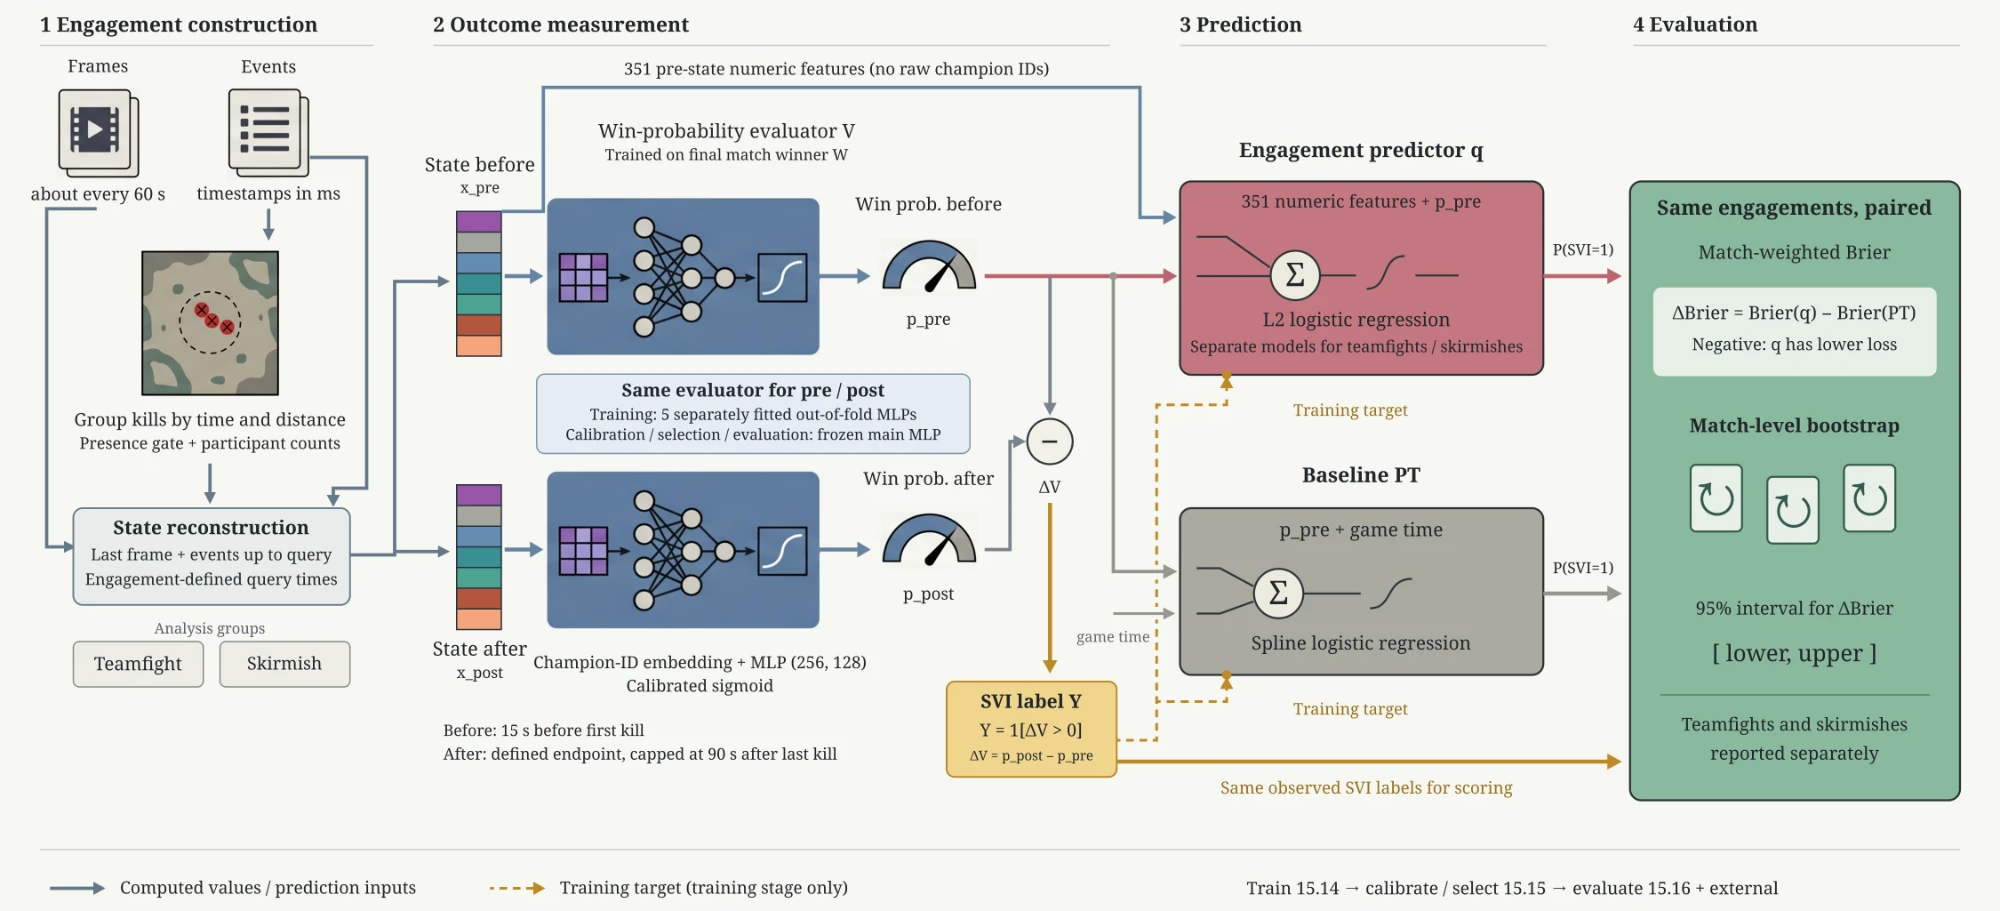
\includegraphics[width=\linewidth]{figures/measure_predict.png}
  \caption{교전 결과의 측정과 방향 예측}
  \label{fig:measure-predict}
\end{sidewaysfigure}

